% -------------------------------------------------------------------------------
% This is all preamble stuff that you don't have to worry about.
% Head down to where it says "Enter your name here"
% -------------------------------------------------------------------------------
 
\documentclass[12pt]{article}
 
\usepackage[margin=1in]{geometry} 
\usepackage{amsmath,amsthm,amssymb}
\usepackage{graphicx}
\usepackage{enumerate}
\usepackage[names]{xcolor}
\usepackage[multiple,hang,flushmargin]{footmisc}
\usepackage{lastpage}


\usepackage[parfill]{parskip}
\parskip=\baselineskip

 
\newenvironment{question}[2][Question]{\begin{trivlist}
\item[\hskip \labelsep {\bfseries #1}\hskip \labelsep {\bfseries #2.}]}{\end{trivlist}}
\newenvironment{solution}[1][Solution:]{\begin{trivlist}
\item[\hskip \labelsep {\bfseries #1}\hskip \labelsep {\bfseries}]\color{blue}}{\end{trivlist}}

\usepackage{fancyhdr}
\pagestyle{fancy}
\rhead{Due: \duedate}
\lhead{CSC250 - Midterm}
\cfoot{p. \thepage \ of \pageref{LastPage}}
\renewcommand{\headrulewidth}{0.4pt}
\renewcommand{\footrulewidth}{0.4pt}

 
\begin{document}
\newcommand{\duedate}{11:59PM EST Thursday March 14, 2024}
 

% --------------------------------------------------------------------------------------------
%  Great, now skip ahead to where you see *** START EXAM HERE ***
% --------------------------------------------------------------------------------------------

\topskip0pt
\vspace*{\fill}
\begin{center}
\fbox{\fbox{\parbox{5.5in}{\begin{center}
\vspace{1em}
This is the first of two examinations for\\ \textbf{CSC250: Theory of Computation}\\ as taught by R. Jordan Crouser and Pablo Frank Bolton in Spring 2024.\\
\vspace{1em}
This exam is \textbf{open book and open note}.\\ The following materials are \textbf{permitted} while taking this examination:
\vspace{1em}
\begin{itemize}
	\item your own notes
	\item lecture slides / videos
	\item scribe notes
	\item homework solutions
	\item any of the recommended textbooks
\end{itemize}
\vspace{1em}
\textbf{Honor code: no other resources are permitted during this exam.}\\
This includes (but is not limited to): online materials, tutors, teaching assistants, and other students.
\end{center}
\vspace{5em}
 \ \ \ YOUR NAME: \underline{\hspace{10cm}}
\vspace{3em}}}}
\end{center}
\vspace{3em}
\vspace*{\fill}


% ---------------------------------------
%   *** START EXAM HERE ***
% ---------------------------------------

\clearpage
\begin{question}{0}\textbf{Getting in the Groove} (0 points)
\begin{center}
\textit{Note: This question is optional, but strongly recommended.}
\end{center}
Educational research studies\footnote{\scriptsize{Lang, Jonas WB, and Jessica Lang. ``Priming competence diminishes the link between cognitive test anxiety and test performance: Implications for the interpretation of test scores.'' \textit{Psychological Science} 21.6 (2010): 811-819.}}\footnote{\scriptsize{Barrows, Jennifer, Samantha Dunn, and Carrie A. Lloyd. ``Anxiety, self-efficacy, and college exam grades.'' \textit{Universal Journal of Educational Research} 1.3 (2013): 204-208.}} have suggested that people perform better on tests when they spend a few minutes thinking about things they're good at before they begin.\\\\
In the space below, briefly tell us about a time when you were \textbf{really successful} at doing something challenging (it doesn't have to be related to this course). If you prefer, you can draw a picture instead of writing.\\
\vfill
\hfill

\includegraphics[width=2in]{youcandoit.png}
\end{question}

% --------
% Logic
% --------
%\clearpage
%\begin{question}{1}\textbf{Propositional logic}\\\\
%Consider the following propositions:
%\begin{eqnarray*}
%	p & = & \texttt{It was raining.}\\
%	q & = & \texttt{We played board games inside.}\\
%	r & = & \texttt{We went to the beach.}
%\end{eqnarray*}
%Translate each of the following propositions into an English sentence.
%\begin{enumerate}[(a)]	
%	\item $q \vee r$\vspace{8em}
%	\item $p \rightarrow q$\vspace{8em}
%	\item $q \rightarrow \neg r$\vspace{8em}
%	\item $p \wedge \neg r \rightarrow q$
%\end{enumerate}
%\end{question}
%
\clearpage
\begin{question}{1}\textbf{Valid or Invalid Reasoning} (6 points)\\\\
For each of the following English arguments, express the argument in terms of
propositional logic and briefly justify whether the argument is valid or invalid. Be sure to clearly label your propositions.
\begin{enumerate}[(a)]	
	\item \textit{When the weather is nice, Max either rides their bike on the rail trail or goes for a walk through the gardens (but never both on the same day). The weather is nice, and Max is going for a walk through the gardens. Therefore, Max will not ride their bike on the rail trail today.}\vspace{16em}
	\item \textit{When students go to Neilson Library, they want to check out a book. No students went to Neilson Library today. This means that no one wanted to check out a book.}
\end{enumerate}
\end{question}

% ---------------------------
% Regular expressions
% ---------------------------
\clearpage
\begin{question}{2}\textbf{Interpreting regular expressions} (3 points)\\\\
Describe the language matched by the following regular expression:
\[0(10)^*1+1(01)^*0\]
\end{question}
\vspace{16em}

\begin{question}{3}\textbf{Writing regular expressions} (3 points)\\\\
Consider the following language on the alphabet $\Sigma = \{0,1\}$:
\[L = \{w \ | \ w \texttt{ has even length, and starts and ends with the same symbol}\}\]
Write a regular expression for $L$.
\end{question}

% ----------------------
% Finite automata
% ----------------------
\clearpage
\begin{question}{4}\textbf{Interpreting  Finite Automata} (4 points)\\\\
Consider the following finite automaton:
\begin{center}
	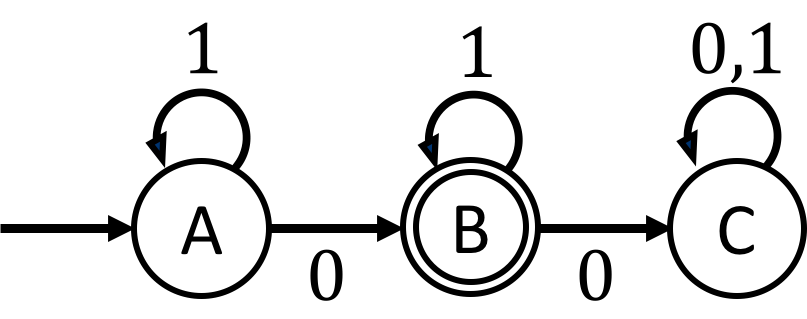
\includegraphics[width=0.6\textwidth]{q4.png}
\end{center}
\begin{enumerate}[(a)]
	\item What is the start state?\vspace{7em}
	\item What is the set of accepting states?\vspace{7em}
	\item Is this a DFA, an NFA, neither, or both?\vspace{7em}
	\item What is the language accepted by this FA?\vspace{7em}
	%\item What sequence of states does this FA go through on input 0011?
\end{enumerate}
\end{question}

\clearpage
\begin{question}{5}\textbf{Building Finite Automata} (6 points)\\\\
Draw the transition diagram for a finite automaton that recognizes each of the following languages. In all cases, the alphabet is $\Sigma = \{0,1\}$.
\begin{enumerate}[(a)]
	\item $\{ w \in \Sigma^* \ | \ w \texttt{ begins with } 1 \texttt{ and ends with } 0 \}$.\vspace{13em}

	\item $\{ w \in \Sigma^* \ | \ w \texttt{ contains an even number of } 1s \}$.\vspace{13em}
	
	\item $\{ w \in \Sigma^* \ | \ w \texttt{ does not contain the substring } 10 \}$.
	
\end{enumerate}
\end{question}


\clearpage
\begin{question}{6}\textbf{Short proofs} (8 points)\\\\
Determine whether each of the following statements is \texttt{true} or \texttt{false}.\\ If it is \texttt{true}, provide a short proof. If it is \texttt{false}, give a counterexample.
\begin{enumerate}[(a)]
\item All regular languages are finite.\vspace{9em}

\item All finite languages are regular.\vspace{9em}

\item All finite automata accept the empty string $\varepsilon$.\vspace{9em}

\item There exists some finite automaton that accepts the empty string $\varepsilon$.

\end{enumerate}
\end{question}

\clearpage
\begin{question}{7}\textbf{Non-Regular Languages} (6 points)\\\\
Prove that the language: \[DOUBLEZERO = \{w \ | \ w \texttt{ contains twice as many } 0s \texttt{ as 1s}\}\] is NOT a regular language.
\end{question}

\clearpage
\begin{question}{8}\textbf{Context-Free Languages} (4 points)\\\\
Prove that the language:
\[DOUBLEZERO= \{w \ | \ w \texttt{ contains twice as many } 0s \texttt{ as 1s}\}\] is context-free.
\end{question}
	

\clearpage
\begin{question}{9}\textbf{Decidable Languages} (4 points)\\\\
Prove that the language:
\[DOUBLEZERO= \{w \ | \ w \texttt{ contains twice as many } 0s \texttt{ as 1s}\}\] is decidable.
\end{question}

\clearpage
\begin{center}
\vspace{-3em}
\textit{This page intentionally left blank as scratch paper.}
\end{center}


% --------------------------------------------------------------
%     You don't have to mess with anything below this line.
% --------------------------------------------------------------
 
\end{document}